\section{WR Transparent Clocks}
\label{sec:wr_tc}
PTP Transparent Clock (TC) modifies PTP messages as they pass through them
adding the residence time of the packet inside of the device. Thus, the delay
introduced  by the network is measured and can be subtracted in the slave clock, 
which improves distribution accuracy.

In ~\ref{sec:wr} the WRPTP and WR synchronization steps has been described for
master, slave and boundary clock. In this chapter the author presents how a TC
uses of the WR synchronization and WRPTP.

\begin{figure*}[!t]
\centering
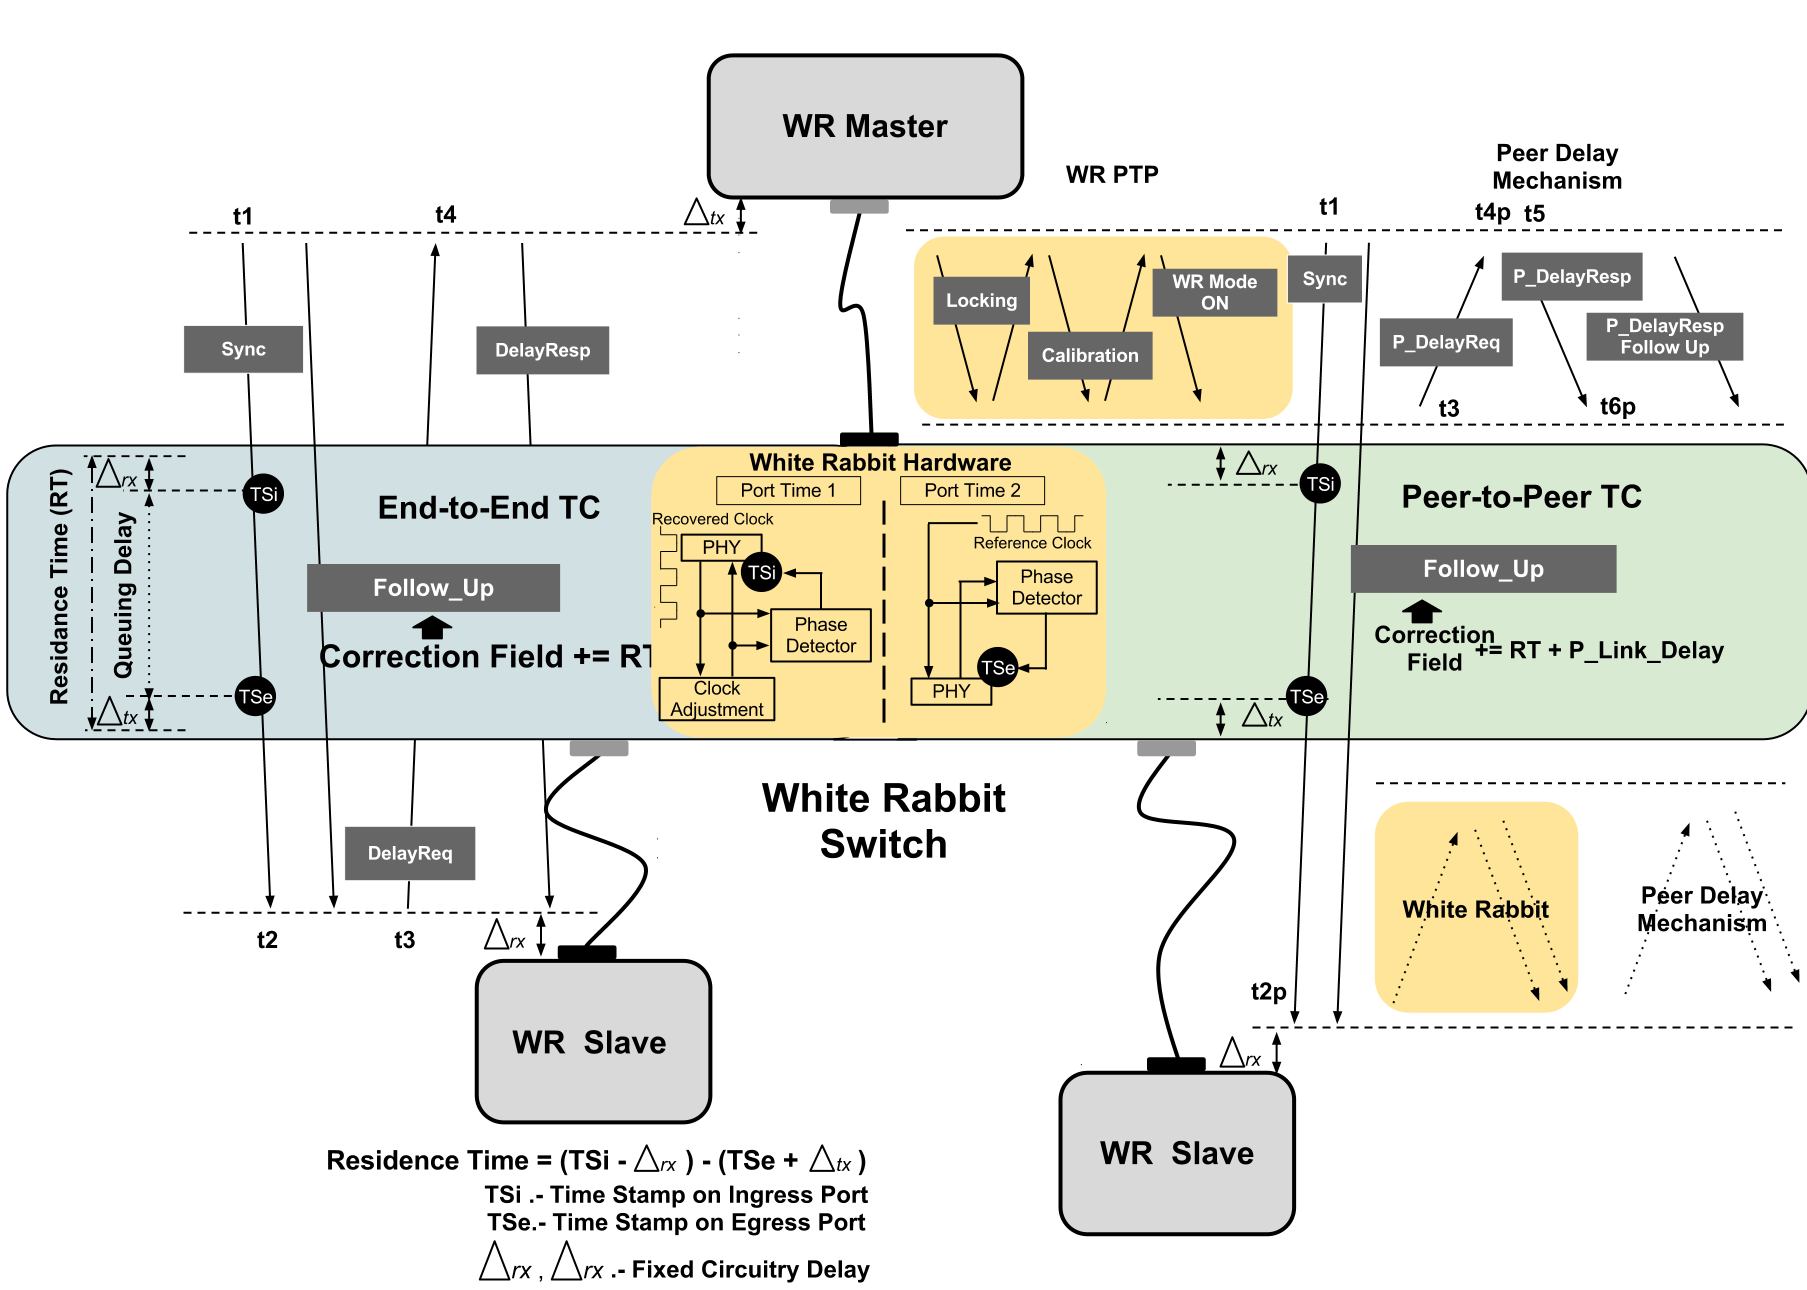
\includegraphics[scale=0.27]{fig/wr_schema_hw_bw.png}
\caption{WR E2E and P2P Transparent Clocks}
\label{fig:wr_tc}
\end{figure*}

\subsection{End-to-End WR Transparent Clock}

As the standard End-to-End (E2E) clocks, the WR E2E TC doesn't belong to the
master-slave hierarchy and does not synchronized to the WR Master. 
Therefore, a WR E2E accomplishes only the synthonization and the calibration,
and not the rest of the steps since the $delay_{ms}$ is calculate end to end,
between master and slave. Thanks to the synthonization there is not errors in
the measurement of the residence time and in the accumulative Correction
Field(CF). In the figure ~\ref{fig:wr_tc} shows the
flow of messages and how the residence time is also calculated taking into account 
the fixed delays $\Delta$. A two-step WR E2E TC calculates, using
(\ref{eq:delayms}), the $offset_{ms}$ \footnote{No enhancement in the timestamps, in chapter
~\ref{sec:issues} this issued will be analyzed}:

\begin{equation}
    \label{eq:wre2e}
     CF += (TS_{ingess\_port} - \Delta_{rx}) -
     (TS_{egress\_port} + \Delta_{tx})
\end{equation}



\begin{equation}
    \label{eq:wre2e}
     offset_{ms} = t_{1} - t_{2} - delay_{ms} - CF
\end{equation}

\subsection{Peer-to-Peer WR Transparent Clock}

As the standard Peer-to-Peer (P2P) clocks, the WR P2P TC measures residence time
of Sync messages, plus the link delay in both directions. Since the link delay
is done between adjacent clocks using the PD mechanism, the fully WR synchronization
process can be issued between ports. The Figure ~\ref{fig:wr_tc} shows how the
WR P2P initiates with the WRPTP one once the WR Mode is on, and continues afterwards doing the
PD mechanism. The steps explained in ~\ref{sec:wr} occurs also in the TC, thanks
to the WR technology. 

The measurement of the residence time, like in the E2E should suffer error
since the port is syntonized to it master clock, but also the measurement of the
link delays as precise as the WR project claims ~\cite{biblio:ispcs_m} for the
Boundary Clocks. The link delay is calculate like in (\ref{eq:delayms}) and the
fig ~\ref{fig:time_stamp} but using $t_{3}$, $t_{4p}$, $t_{5}$ and $t_{6p}$. 
The $offset_{ms}$ is calculated :


\begin{equation}
    \label{eq:wre2e}
     CF += residance\_time + delay\_link
\end{equation}


\begin{equation}
    \label{eq:wre2e}
     offset_{ms}= t_{1} - t_{2} - CF - delay\_link \footnote{This link delay
     correspond to the las link to the slave}
\end{equation}



\FloatBarrier
